\documentclass[11pt,a4paper]{article}
\usepackage[margin={2.6cm,2.6cm}]{geometry}
\usepackage{lmodern}
\usepackage{microtype}
\usepackage{enumitem}
\usepackage{array}
\usepackage[spanish,es-tabla]{babel}
\usepackage[utf8]{inputenc}
\usepackage[T1]{fontenc}
\usepackage{amsmath, amsthm}
\usepackage{hyperref}
\usepackage{xcolor}
\usepackage{graphicx}
\usepackage{listings}
\usepackage{fontawesome5}
\usepackage{dirtree}


\definecolor{azuluc}{HTML}{1F4E79}
\definecolor{grisclaro}{HTML}{F4F6F8}
\definecolor{gris}{HTML}{586069}
\definecolor{verde}{HTML}{2E7D32}
\definecolor{rojo}{HTML}{A94442}
\definecolor{git}{HTML}{F1502F}

\definecolor{morado_ubuntu}{RGB}{48, 10, 36}       % Fondo morado oscuro de Ubuntu GNOME
\definecolor{verde_ubuntu}{RGB}{78, 154, 6}        % Verde para comentarios
\definecolor{cyan_ubuntu}{RGB}{52, 226, 226}       % Cian para comandos
\definecolor{amarillo_ubuntu}{RGB}{250, 240, 190}  % Amarillo para cadenas
\definecolor{rojo_ubuntu}{RGB}{220, 50, 47}        % Rojo para errores
\definecolor{verde_claro_ubuntu}{RGB}{138, 226, 52} % Verde claro para el prompt
\definecolor{azul_ubuntu}{RGB}{114, 159, 207}      % Azul para símbolos y rutas
\definecolor{gris_ubuntu}{RGB}{128, 128, 128}      % Gris para el borde del frame


\definecolor{fondo_mac}{RGB}{255, 255, 250}       % Fondo beige claro típico de macOS
\definecolor{negro}{RGB}{0, 0, 0}                 % Texto en negro
\definecolor{verde_mac}{RGB}{63, 127, 95}         % Verde para comentarios
\definecolor{azul_mac}{RGB}{0, 0, 255}            % Azul para comandos y prompt
\definecolor{rojo_mac}{RGB}{196, 26, 22}          % Rojo para errores y cadenas
\definecolor{morado_mac}{RGB}{147, 39, 143}       % Morado para emphasis (opcional)
\definecolor{gris_mac}{RGB}{200, 200, 200}        % Gris para el borde del frame



\lstdefinestyle{rstyle}{
  language=R,
  basicstyle=\ttfamily\small,
  keywordstyle=\color{azuluc}\bfseries,
  commentstyle=\color{gris},
  stringstyle=\color{verde!70!black},
  showstringspaces=false,
  frame=single,
  rulecolor=\color{gris!30},
  backgroundcolor=\color{grisclaro},
  breaklines=true,
  showspaces=false,
  tabsize=2
}

\lstdefinestyle{rconsole}{
  language=R,
  basicstyle=\color{rojo}\ttfamily\small,
  showstringspaces=false,
  columns=fullflexible,
  frame=single,
  rulecolor=\color{gris!30},
  breaklines=true,
  tabsize=2
}

\lstdefinestyle{routput}{
  language=R,
  basicstyle=\color{azuluc}\ttfamily\small,
  showstringspaces=false,
  columns=fullflexible,
  frame=single,
  rulecolor=\color{gris!30},
  breaklines=true,
  tabsize=2
}

\lstdefinestyle{mdstyle}{
  basicstyle=\ttfamily\footnotesize,
  keywordstyle=\color{azuluc}\bfseries,
  commentstyle=\color{gris},
  showstringspaces=false,
  showspaces=false,
  tabsize=2,
  frame=single,
  rulecolor=\color{gris!30},
  backgroundcolor=\color{grisclaro},
  breaklines=true,
  breakatwhitespace=false,
  % Títulos Markdown
  morecomment=[l][\color{azuluc}\bfseries]{\#},
  % Enlaces y referencias
  morecomment=[s][\color{verde}]{(}{)},
  % Cadenas
  morestring=[b][\color{naranja}]{"},
  morestring=[b][\color{naranja}]{'},
  % Lenguajes utilizados en bloques de código
  classoffset=1,
    keywordstyle=\color{morado}\bfseries,
    morekeywords={python,bash,R,latex,json,yaml},
  classoffset=0,
  % Protocolos y enlaces
  emph={http,https,ftp},
  escapeinside={-@}{@-},
  emphstyle=\color{azuluc}\underbar,   
   literate=
    {á}{{\'a}}1
    {é}{{\'e}}1
    {í}{{\'i}}1
    {ó}{{\'o}}1
    {ú}{{\'u}}1
    {Á}{{\'A}}1
    {É}{{\'E}}1
    {Í}{{\'I}}1
    {Ó}{{\'O}}1
    {Ú}{{\'U}}1
    {ñ}{{\~n}}1
    {Ñ}{{\~N}}1
    {ü}{{\"u}}1
    {Ü}{{\"U}}1
    {¡}{{\textexclamdown}}1
	{`}{\textasciigrave}1 
    {´}{\textquotesingle}1,
}

\lstdefinestyle{ubuntugnome}{
  basicstyle=\ttfamily\small\color{white},
  backgroundcolor=\color{morado_ubuntu},
  commentstyle=\color{verde_ubuntu},
  keywordstyle=\color{cyan_ubuntu},
  stringstyle=\color{amarillo_ubuntu},
  emphstyle=\color{rojo_ubuntu},
  showstringspaces=false,
  frame=single,
  rulecolor=\color{gris_ubuntu},
  breaklines=true,
  postbreak=\mbox{\textcolor{white}{$\hookrightarrow$}\space},
  % Configuración para simular el prompt de Ubuntu
  upquote=true,
  % Resaltar el prompt de usuario
  emph={user@ubuntu:~\$},
  emphstyle={\color{verde_claro_ubuntu}\bfseries},
  % Resaltar errores (ej: "command not found")
  classoffset=1,
  emph={command not found,No such file or directory,Permission denied},
  emphstyle={\color{rojo_ubuntu}},
  classoffset=0,
}

\lstdefinestyle{macterminal}{
  basicstyle=\ttfamily\small\color{negro},
  backgroundcolor=\color{fondo_mac},
  commentstyle=\color{verde_mac},
  keywordstyle=\color{azul_mac},
  stringstyle=\color{rojo_mac},
  emphstyle=\color{morado_mac},
  showstringspaces=false,
  frame=single,
  rulecolor=\color{gris_mac},
  breaklines=true,
  postbreak=\mbox{\textcolor{negro}{$\hookrightarrow$}\space},
  % Configuración para simular el prompt de macOS
  upquote=true,
  % Resaltar el prompt de usuario
  emphstyle={\color{azul_mac}\bfseries},
  % Resaltar errores (ej: "command not found")
  classoffset=1,
  emph={command not found,No such file or directory,Permission denied},
  emphstyle={\color{rojo_mac}},
  classoffset=0
}

\lstdefinestyle{windowscmd}{
  basicstyle=\ttfamily\small\color{white},
  backgroundcolor=\color{black},
  showstringspaces=false,
  frame=single,
  rulecolor=\color{gris_mac},
  breaklines=true,
  postbreak=\mbox{\textcolor{negro}{$\hookrightarrow$}\space},
  % Configuración para simular el prompt de macOS
  upquote=true,
  % Resaltar el prompt de usuario
  emphstyle={\color{azul_mac}\bfseries},
  % Resaltar errores (ej: "command not found")
  classoffset=1,
  emph={command not found,No such file or directory,Permission denied},
  emphstyle={\color{rojo_mac}},
  classoffset=0
}



\newcommand*{\vsp}{\texttt{\textvisiblespace}} % visible space

\newcommand*{\strC}{\begingroup
  \obeyspaces
  \begingroup\lccode`~=`\ %
  \lowercase{\endgroup\let~}\vsp
  \dostrC}
\newcommand{\dostrC}[1]{\textnormal{{\slshape\ttfamily#1}}\endgroup} % string constant


\newcommand{\R}{\textcolor{azuluc}{\faIcon{r-project}}}
\newcommand{\Git}{\textcolor{git}{\faIcon{git-alt}}~\!Git}
\newcommand{\GitHub}{\faIcon{github}~\!GitHub}
\newcommand{\Markdown}{Markdown~\faIcon{markdown}}



\newcommand{\checkicon}{\textcolor{verde}{\faIcon{check}}}
\newcommand{\crossicon}{\textcolor{rojo}{\faIcon{times}}}

\newtheoremstyle{exercise}
  {0.8em}{0.8em}{\normalfont}{}{\bfseries\color{azuluc}}{.}{0.5em}{}
\theoremstyle{exercise}
\newtheorem{exercise}{Ejercicio}


\title{\LARGE \textbf{Práctica 4: Introducción a \Markdown} \\[0.5em]
\Large Laboratorio de Matemáticas \\
\small \ \\
Grado en Ingeniería Matemática - Doble Grado en Física e Ingeniería Matemática}
\author{Miguel Beltra Vidal}
\date{Curso 2026/27}

\begin{document}

\maketitle


\section{Objetivos}

El objetivo de esta práctica es introducir la sintaxis básica del lenguaje de marcado \Markdown. Al finalizarla, el estudiante será capaz de escribir documentación usando este lenguaje.

 

\section{Introducción}

El contenido de estas primeras páginas es una traducción del apartado \textbf{Basic Syntax} que se puede encontrar en 
\begin{center}
	\url{https://www.markdownguide.org/basic-syntax/},
\end{center}
además de algunos añadidos que se han considerado oportunos.

\medskip

Casi todas las aplicaciones de \Markdown\ admiten la sintaxis básica descrita en el documento de diseño original de \Markdown. Existen pequeñas variaciones y discrepancias entre los distintos procesadores de \Markdown; siempre que es posible, se indican en el propio texto. Algunas herramientas para poder previsualizar un fichero escrito en \Markdown\ son:
\begin{itemize}
	\item \url{https://markdownviewer.pages.dev/}
	\item \url{https://markdownlivepreview.com/}
	\item \url{https://markdownlivepreview.dev/}
\end{itemize}


\section{Organización}

\subsection{Encabezados}

Para crear un encabezado, añade almohadillas (\verb|#|) delante de una palabra o frase. El número de almohadillas que utilices debe corresponder al nivel del encabezado. Por ejemplo, para crear un encabezado de nivel tres, utiliza tres almohadillas (por ejemplo, \verb|### Mi encabezado|).

\bigskip

\noindent
\begin{minipage}{0.5\textwidth}
\begin{lstlisting}[style=mdstyle]
# Encabezado de nivel 1

## Encabezado de nivel 2

### Encabezado de nivel 3

#### Encabezado de nivel 4

##### Encabezado de nivel 5

###### Encabezado de nivel 6
\end{lstlisting}
\end{minipage}
~
\begin{minipage}{0.475\textwidth}
	\vfill
	\quad~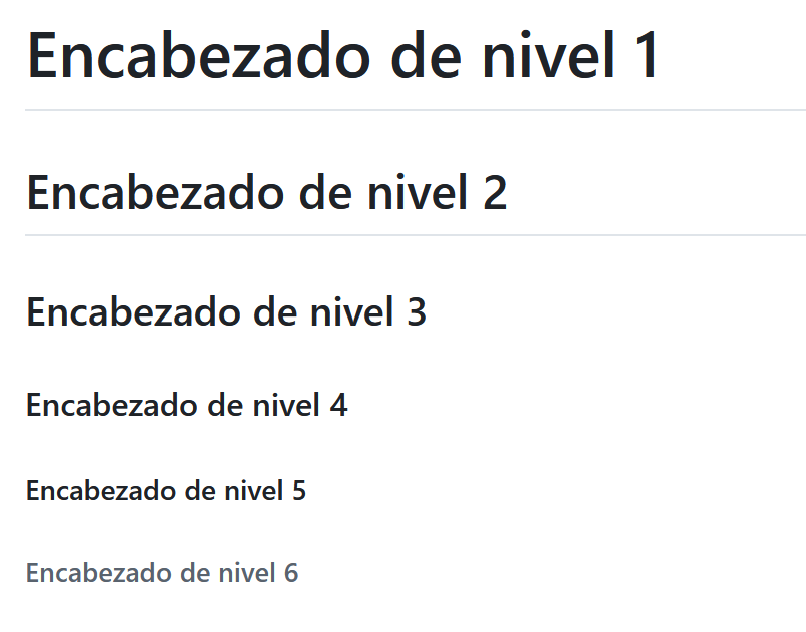
\includegraphics[scale=0.7]{images/headings_1}
	\vfill
\end{minipage}


\noindent Como alternativa, en la línea situada debajo del texto, añade cualquier número de caracteres \verb|==| para un encabezado de nivel 1 o \verb|--| para un encabezado de nivel 2.

\bigskip


\noindent
\begin{minipage}{0.5\textwidth}
\begin{lstlisting}[style=mdstyle]
Encabezado de nivel 1
======================

Encabezado de nivel 2
----------------------
\end{lstlisting}
\end{minipage}
~
\begin{minipage}{0.475\textwidth}
	\vfill
	\quad~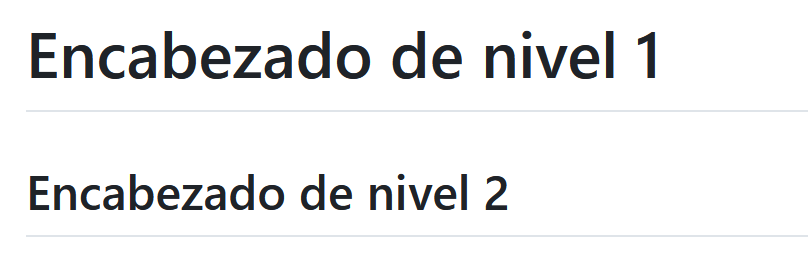
\includegraphics[scale=0.7]{images/headings_2}
	\vfill
\end{minipage}




\subsubsection{Buenas prácticas para los encabezados}

Las aplicaciones de Markdown no se ponen de acuerdo sobre cómo gestionar la ausencia de un espacio entre las almohadillas (\verb|#|) y el nombre del encabezado. Por compatibilidad, pon siempre un espacio entre las almohadillas y el nombre del encabezado.

\begin{center}
\begin{tabular}{|p{0.45\textwidth}|p{0.45\textwidth}|} \hline
	\checkicon\ Haz esto & \crossicon\ No hagas esto \\ \hline
	& \\
	\verb|# Este es un encabezado| & \verb|#Este es un encabezado| \\
	& \\ \hline
\end{tabular}
\end{center}


\noindent También deberías dejar líneas en blanco antes y después de un encabezado para garantizar la compatibilidad.

\begin{center}
\begin{tabular}{|p{0.45\textwidth}|p{0.45\textwidth}|} \hline
	\checkicon\ Haz esto & \crossicon\ No hagas esto \\ \hline
	
	\begin{tabular}{l}
		\\
		\verb|Pon una línea en blanco antes...| \\
		\\
		\verb|# Encabezado| \\
		\\
		\verb|... y después de un encabezado.| \\
		\\
	\end{tabular}		
	& 
	\begin{tabular}{l}
		\\
		\verb|Sin líneas en blanco...| \\
		\verb|# Encabezado| \\
		\verb|... podría no verse correctamente.| \\
		\\
		\\
		\\
	\end{tabular}
	\\ \hline
\end{tabular}
\end{center}



\subsection{Párrafos}

Para crear párrafos, utiliza una línea en blanco para separar una o más líneas de texto.

\bigskip

\noindent
\begin{minipage}{0.5\textwidth}
\begin{lstlisting}[style=mdstyle]
Me gusta mucho utilizar Markdown.

Lo utilizaré para dar formato a todos 
mis documentos.
\end{lstlisting}
\end{minipage}
~
\begin{minipage}{0.475\textwidth}
	\vfill
	\quad~
\includegraphics[scale=0.7]{images/paragraph}
	\vfill
\end{minipage}




\subsubsection{Buenas prácticas para los párrafos}

Si el párrafo no está dentro de una lista, no indentes los párrafos con espacios o tabuladores.

\begin{center}
\begin{tabular}{|l|l|} \hline
	\checkicon\ Haz esto & \crossicon\ No hagas esto \\ \hline
	
	\begin{tabular}{l}
		\\
		\verb|No pongas tabuladores ni espacios| \\
		\verb|delante de los párrafos. Mantén las| \\
		\verb|líneas alineadas a la izquierda de| \\
		\verb|esta manera.| \\
		\\
	\end{tabular}
	&
	\begin{tabular}{l}
		\\
		\verb|    Esto puede provocar problemas| \\
		\verb|de formato inesperados. No añadas| \\
		\verb|tabuladores ni espacios delante| \\
		\verb|de los párrafos.| \\
		\\
	\end{tabular}
	 \\ \hline
\end{tabular}
\end{center}


%\noindent\textbf{Nota:} Para indentar párrafos en el resultado, consulta la sección sobre cómo indentar (tabulador).


\subsection{Saltos de línea}

Para crear un salto de línea o una nueva línea, termina una línea con dos o más espacios y, a continuación, pulsa Intro. En el siguiente ejemplo se muestran los espacios de forma explícita con el carácter \vsp.

\bigskip

\noindent
\begin{minipage}{0.5\textwidth}
\begin{lstlisting}[style=mdstyle,showspaces=true]
Primera línea.-@\vsp\vsp@-
Segunda línea.
\end{lstlisting}
\end{minipage}
~
\begin{minipage}{0.475\textwidth}
	\vfill
	\quad~
\includegraphics[scale=0.7]{images/newline}
	\vfill
\end{minipage}




\subsection{Buenas prácticas para los saltos de línea}

Puedes utilizar dos o más espacios (lo que normalmente se denomina «espacio en blanco final») para crear saltos de línea en prácticamente cualquier aplicación de \Markdown, pero es un método controvertido. Es difícil ver los espacios finales en un editor y muchas personas añaden accidental o intencionadamente dos espacios después de cada frase. Por este motivo, quizá quieras utilizar otra opción para los saltos de línea. Si tu aplicación de \Markdown\ admite HTML, puedes utilizar la etiqueta HTML \texttt{<br>}. 

Hay otras dos opciones. CommonMark y algunos otros lenguajes ligeros de marcado permiten escribir una barra invertida (\verb|\|) al final de la línea, pero no todas las aplicaciones de \Markdown\ lo admiten, por lo que no es una buena opción desde el punto de vista de la compatibilidad.


\begin{center}
\begin{tabular}{|l|l|} \hline
	\checkicon\ Haz esto & \crossicon\ No hagas esto \\ \hline
	
	\begin{tabular}{l}
		\\
		\verb|Línea con dos espacios después.|\vsp\vsp \\
		\verb|Y siguiente línea| \\
		\\
		\verb|Línea con etiqueta HTML después.<br>| \\
		\verb|Y siguiente línea| \\
		\\
	\end{tabular}
	&
	\begin{tabular}{l}
		\\
		\verb|Línea con barra después.\| \\
		\verb|Y siguiente línea| \\
		\\
		\verb|Línea sin nada después.| \\
		\verb|Y siguiente línea| \\
		\\
	\end{tabular}
	 \\ \hline
\end{tabular}
\end{center}








\section{Énfasis}

Puedes añadir énfasis haciendo que el texto aparezca en \emph{cursiva} o \textbf{negrita}.

\subsection{Cursiva}

Para poner un texto en cursiva, añade un asterisco o un guion bajo antes y después de una palabra o frase. Para poner en cursiva la parte central de una palabra, añade un asterisco sin espacios alrededor de las letras.

\bigskip

\noindent
\begin{minipage}{0.5\textwidth}
\begin{lstlisting}[style=mdstyle]
La cursiva es *lo más de lo más*.

La cursiva es _lo más de lo más_.

Lo*mas*delo*mas*.
\end{lstlisting}
\end{minipage}
~
\begin{minipage}{0.475\textwidth}
	\vfill
	\quad~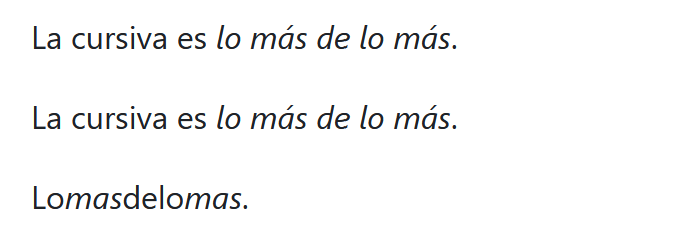
\includegraphics[scale=0.7]{images/italic}
	\vfill
\end{minipage}



\subsubsection{Buenas prácticas para la cursiva}

Las aplicaciones de Markdown no se ponen de acuerdo sobre cómo gestionar los guiones bajos en el centro de una palabra. Por compatibilidad, utiliza asteriscos para poner en cursiva la parte central de una palabra.

\begin{center}
\begin{tabular}{|p{0.45\textwidth}|p{0.45\textwidth}|} \hline
	\checkicon\ Haz esto & \crossicon\ No hagas esto \\ \hline
	
	\begin{tabular}{l}
		\\
		\verb|Lo*mas*delo*mas*.           | \\
		\\
	\end{tabular}
	&
	\begin{tabular}{l}
		\\
		\verb|Lo_mas_delo_mas_.           | \\
		\\
	\end{tabular}
	 \\ \hline
\end{tabular}
\end{center}

\subsection{Negrita}

Para poner un texto en negrita, añade dos asteriscos o guiones bajos antes y después de una palabra o frase. Para poner en negrita la parte central de una palabra, añade dos asteriscos sin espacios alrededor de las letras.

\bigskip

\noindent
\begin{minipage}{0.5\textwidth}
\begin{lstlisting}[style=mdstyle]
Me encanta el **texto en negrita**.

Me encanta el __texto en negrita__.

Amo**la**negrita.
\end{lstlisting}
\end{minipage}
~
\begin{minipage}{0.475\textwidth}
	\vfill
	\quad~
\includegraphics[scale=0.7]{images/bold}
	\vfill
\end{minipage}



\subsubsection{Buenas prácticas para la negrita}

Las aplicaciones de Markdown no se ponen de acuerdo sobre cómo gestionar los guiones bajos en el centro de una palabra. Por compatibilidad, utiliza asteriscos para poner en negrita la parte central de una palabra.

\begin{center}
\begin{tabular}{|p{0.45\textwidth}|p{0.45\textwidth}|} \hline
	\checkicon\ Haz esto & \crossicon\ No hagas esto \\ \hline
	
	\begin{tabular}{l}
		\\
		\verb|Amo**la**negrita           | \\
		\\
	\end{tabular}
	&
	\begin{tabular}{l}
		\\
		\verb|Amo__la__negrita           | \\
		\\
	\end{tabular}
	 \\ \hline
\end{tabular}
\end{center}


\subsection{Negrita y cursiva}

Para enfatizar un texto con negrita y cursiva al mismo tiempo, añade tres asteriscos o guiones bajos antes y después de una palabra o frase. Para poner en negrita y cursiva la parte central de una palabra, añade tres asteriscos sin espacios alrededor de las letras.

\bigskip

\noindent
\begin{minipage}{0.5\textwidth}
\begin{lstlisting}[style=mdstyle]
Texto ***realmente importante***.

Texto ___realmente importante___.

Texto __*realmente importante*__.

Texto **_realmente importante_**.

Texto realmente***muy***importante.
\end{lstlisting}
\end{minipage}
~
\begin{minipage}{0.475\textwidth}
	\vfill
	\quad~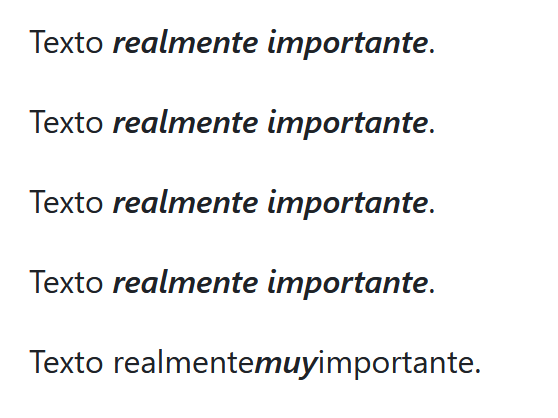
\includegraphics[scale=0.7]{images/italic_bold}
	\vfill
\end{minipage}







\subsubsection{Buenas prácticas para negrita y cursiva}

Las aplicaciones de Markdown no se ponen de acuerdo sobre cómo gestionar los guiones bajos en el centro de una palabra. Por compatibilidad, utiliza asteriscos para poner en negrita y cursiva la parte central de una palabra.

\begin{center}
\begin{tabular}{|l|l|} \hline
	\checkicon\ Haz esto & \crossicon\ No hagas esto \\ \hline
	
	\begin{tabular}{l}
		\\
		\verb|Texto realmente***muy***importante.| \\
		\\
	\end{tabular}
	&
	\begin{tabular}{l}
		\\
		\verb|Text realmente___muy___importante.| \\
		\\
	\end{tabular}
	 \\ \hline
\end{tabular}
\end{center}




\subsection{Citas en bloque}

Para crear una cita en bloque, añade un \texttt{>} delante de un párrafo.

\medskip

\begin{lstlisting}[style=mdstyle]
> Dorothy la siguió por muchas de las hermosas habitaciones de su castillo.
\end{lstlisting}

\noindent El resultado se muestra así:

%> Dorothy la siguió por muchas de las hermosas habitaciones de su castillo.

\bigskip


\includegraphics[scale=0.7]{images/blockquote_1}


\subsubsection{Citas en bloque con varios párrafos}

Las citas en bloque pueden contener varios párrafos. Añade un \texttt{>} en las líneas en blanco entre los párrafos.

\medskip

\begin{lstlisting}[style=mdstyle]
> Dorothy la siguió por muchas de las hermosas habitaciones de su castillo.
>
> La Bruja le ordenó limpiar las ollas y las cacerolas, barrer el suelo y
mantener el fuego alimentado con leña.
\end{lstlisting}

\noindent El resultado se muestra así:

%> Dorothy la siguió por muchas de las hermosas habitaciones de su castillo.
%>
%> La Bruja le ordenó limpiar las ollas y las cacerolas, barrer el suelo y mantener el fuego alimentado con leña.

\bigskip


\includegraphics[scale=0.7]{images/blockquote_2}


\subsubsection{Citas en bloque anidadas}

Las citas en bloque pueden anidarse. Añade \texttt{>}\texttt{>} delante del párrafo que quieras anidar.

\medskip

\begin{lstlisting}[style=mdstyle]
> Dorothy la siguió por muchas de las hermosas habitaciones de su castillo.
>
>> La Bruja le ordenó limpiar las ollas y las cacerolas, barrer el suelo y 
mantener el fuego alimentado con leña.
\end{lstlisting}

\noindent El resultado se muestra así:

%> Dorothy la siguió por muchas de las hermosas habitaciones de su castillo.
%>
%> > La Bruja le ordenó limpiar las ollas y las cacerolas, barrer el suelo y mantener el fuego alimentado con leña.

\bigskip

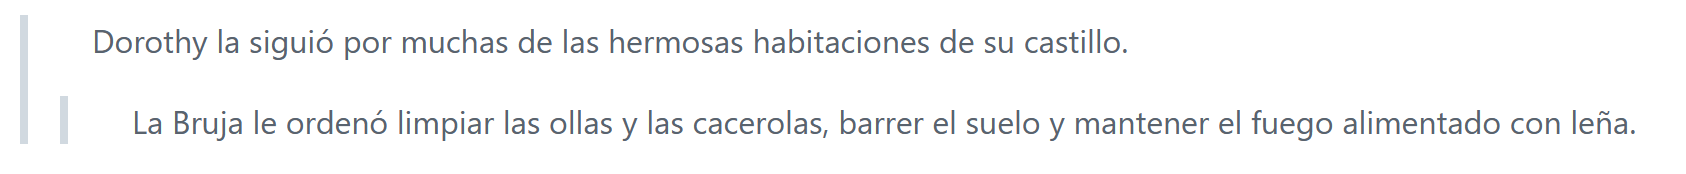
\includegraphics[scale=0.7]{images/blockquote_3}


\subsubsection{Citas en bloque con otros elementos}

Las citas en bloque pueden contener otros elementos de Markdown con formato. No todos los elementos pueden utilizarse; tendrás que experimentar para comprobar cuáles funcionan.

\medskip

\begin{lstlisting}[style=mdstyle]
> #### Los resultados trimestrales tienen muy buen aspecto.
>
> - Los ingresos se dispararon.
> - Los beneficios fueron más altos que nunca.
>
> *Todo* va de acuerdo con el **plan**.
\end{lstlisting}

\noindent El resultado se muestra así:

%> #### Los resultados trimestrales tienen muy buen aspecto.
%>
%> * Los ingresos se dispararon.
%> * Los beneficios fueron más altos que nunca.
%>
%> *Todo* va de acuerdo con el **plan**.

\bigskip

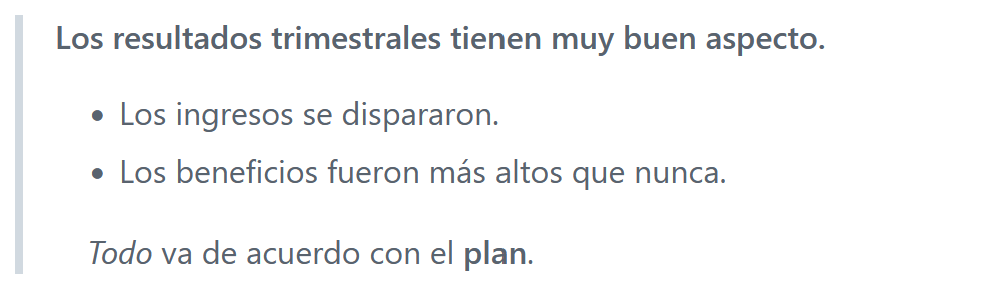
\includegraphics[scale=0.7]{images/blockquote_4}


\subsubsection{Buenas prácticas para las citas en bloque}

Por compatibilidad, deja líneas en blanco antes y después de las citas en bloque.

\begin{center}
\begin{tabular}{|l|l|} \hline
	\checkicon\ Haz esto & \crossicon\ No hagas esto \\ \hline
	
	\begin{tabular}{l}
		\\
		\verb|Pon una línea en blanco antes...| \\
		\\
		\verb|> Esta es una cita en bloque| \\
		\\
		\verb|...y después de una cita en bloque.| \\
		\\
	\end{tabular}
	&
	\begin{tabular}{l}
		\\
		\verb|Sin líneas en blanco, esto| \\
		\verb|podría no verse correctamente.   | \\
		\verb|> Esta es una cita en bloque| \\
		\verb|¡No hagas esto!| \\
		\\
		\\
	\end{tabular}
	 \\ \hline
\end{tabular}
\end{center}





\section{Listas}

Puedes organizar elementos mediante listas ordenadas y no ordenadas.


\subsection{Listas ordenadas}

Para crear una lista ordenada, añade elementos precedidos por números y puntos. Los números no tienen que estar en orden numérico, pero la lista debe comenzar con el número uno.

\medskip

\noindent
\begin{minipage}{0.5\textwidth}
\begin{lstlisting}[style=mdstyle]
1. Primer elemento
2. Segundo elemento
3. Tercer elemento
4. Cuarto elemento
\end{lstlisting}
\end{minipage}
~
\begin{minipage}{0.475\textwidth}
	\vfill
	\quad~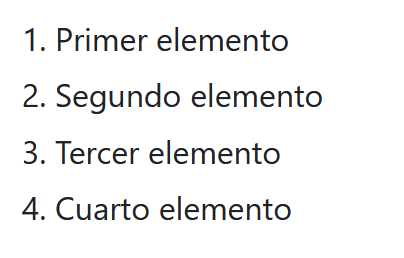
\includegraphics[scale=0.7]{images/ordered_list_1}
	\vfill
\end{minipage}

%1. Primer elemento
%2. Segundo elemento
%3. Tercer elemento
%4. Cuarto elemento

\bigskip

\noindent También puedes utilizar siempre el número 1:

\medskip

\noindent
\begin{minipage}{0.5\textwidth}
\begin{lstlisting}[style=mdstyle]
1. Primer elemento
1. Segundo elemento
1. Tercer elemento
1. Cuarto elemento
\end{lstlisting}
\end{minipage}
~
\begin{minipage}{0.475\textwidth}
	\vfill
	\quad~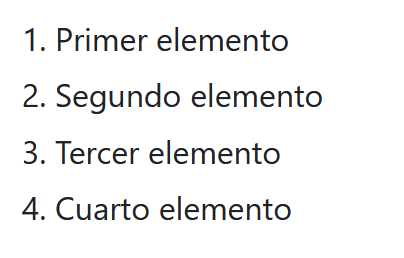
\includegraphics[scale=0.7]{images/ordered_list_1}
	\vfill
\end{minipage}

%El resultado será:
%1. Primer elemento
%2. Segundo elemento
%3. Tercer elemento
%4. Cuarto elemento


\bigskip

\noindent También puedes utilizar números que no estén en orden:

\medskip

\noindent
\begin{minipage}{0.5\textwidth}
\begin{lstlisting}[style=mdstyle]
1. Primer elemento
8. Segundo elemento
3. Tercer elemento
5. Cuarto elemento
\end{lstlisting}
\end{minipage}
~
\begin{minipage}{0.475\textwidth}
	\vfill
	\quad~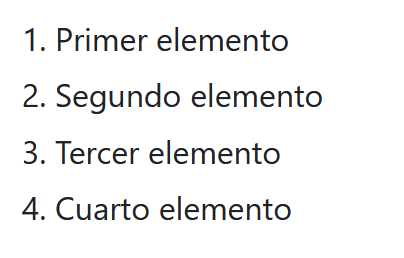
\includegraphics[scale=0.7]{images/ordered_list_1}
	\vfill
\end{minipage}

%El resultado será:
%1. Primer elemento
%2. Segundo elemento
%3. Tercer elemento
%4. Cuarto elemento


\bigskip

\noindent Puedes crear listas anidadas indentando los elementos:

\medskip

\noindent
\begin{minipage}{0.5\textwidth}
\begin{lstlisting}[style=mdstyle]
1. Primer elemento
2. Segundo elemento
3. Tercer elemento
    1. Elemento indentado
    2. Elemento indentado
4. Cuarto elemento
\end{lstlisting}
\end{minipage}
~
\begin{minipage}{0.475\textwidth}
	\vfill
	\quad~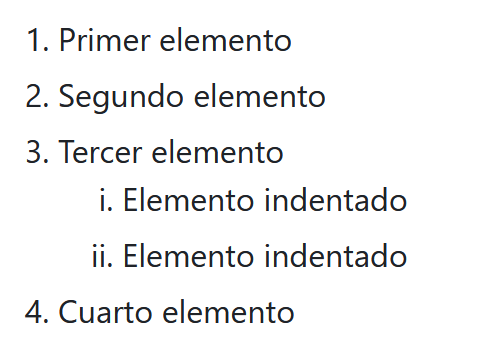
\includegraphics[scale=0.7]{images/ordered_list_2}
	\vfill
\end{minipage}

%El resultado será:
%1. Primer elemento
%2. Segundo elemento
%3. Tercer elemento
%
%   1. Elemento indentado
%   2. Elemento indentado
%4. Cuarto elemento




\subsubsection{Buenas prácticas para las listas ordenadas}

CommonMark y algunos otros lenguajes ligeros de marcado permiten utilizar un paréntesis (\texttt{)}) como delimitador (por ejemplo, \verb|1) Primer elemento|), pero no todas las aplicaciones de Markdown lo admiten, por lo que no es una buena opción desde el punto de vista de la compatibilidad. Por compatibilidad, utiliza únicamente puntos.



\begin{center}
\begin{tabular}{|p{0.45\textwidth}|p{0.45\textwidth}|} \hline
	\checkicon\ Haz esto & \crossicon\ No hagas esto \\ \hline
	
	\begin{tabular}{l}
		\\
		\verb|1. Primer elemento      | \\
		\verb|2. Segundo elemento     | \\
		\\
	\end{tabular}
	&
	\begin{tabular}{l}
		\\
		\verb|1) Primer elemento      | \\
		\verb|2) Segundo elemento     | \\
		\\
	\end{tabular}
	 \\ \hline
\end{tabular}
\end{center}





\subsection{Listas no ordenadas}

Para crear una lista no ordenada, añade guiones (\texttt{-}), asteriscos (\texttt{*}) o signos más (\texttt{+}) delante de los elementos. Indenta uno o más elementos para crear una lista anidada.

\medskip

\noindent
\begin{minipage}{0.5\textwidth}
\begin{lstlisting}[style=mdstyle]
- Primer elemento
- Segundo elemento
- Tercer elemento
- Cuarto elemento
\end{lstlisting}
\end{minipage}
~
\begin{minipage}{0.475\textwidth}
	\vfill
	\quad~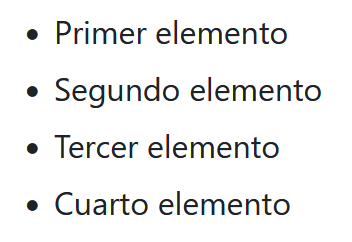
\includegraphics[scale=0.7]{images/unordered_list_1}
	\vfill
\end{minipage}

%El resultado será:
%* Primer elemento
%* Segundo elemento
%* Tercer elemento
%* Cuarto elemento

\bigskip



\noindent También puedes utilizar asteriscos:

\medskip

\noindent
\begin{minipage}{0.5\textwidth}
\begin{lstlisting}[style=mdstyle]
* Primer elemento
* Segundo elemento
* Tercer elemento
* Cuarto elemento
\end{lstlisting}
\end{minipage}
~
\begin{minipage}{0.475\textwidth}
	\vfill
	\quad~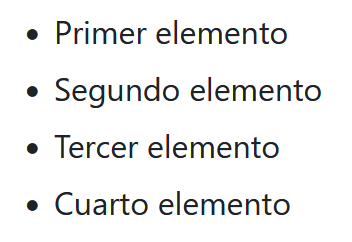
\includegraphics[scale=0.7]{images/unordered_list_1}
	\vfill
\end{minipage}

%El resultado será:
%* Primer elemento
%* Segundo elemento
%* Tercer elemento
%* Cuarto elemento

\bigskip


\noindent O signos más:

\medskip

\noindent
\begin{minipage}{0.5\textwidth}
\begin{lstlisting}[style=mdstyle]
+ Primer elemento
+ Segundo elemento
+ Tercer elemento
+ Cuarto elemento
\end{lstlisting}
\end{minipage}
~
\begin{minipage}{0.475\textwidth}
	\vfill
	\quad~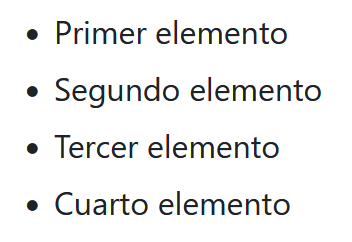
\includegraphics[scale=0.7]{images/unordered_list_1}
	\vfill
\end{minipage}

%El resultado será:
%* Primer elemento
%* Segundo elemento
%* Tercer elemento
%* Cuarto elemento

\bigskip



\noindent Para crear una lista anidada:

\medskip

\noindent
\begin{minipage}{0.5\textwidth}
\begin{lstlisting}[style=mdstyle]
- Primer elemento
- Segundo elemento
- Tercer elemento
    - Elemento indentado
    - Elemento indentado
- Cuarto elemento
\end{lstlisting}
\end{minipage}
~
\begin{minipage}{0.475\textwidth}
	\vfill
	\quad~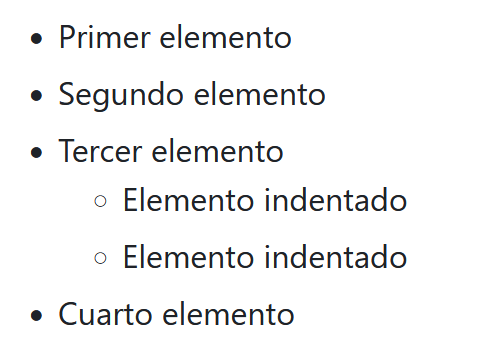
\includegraphics[scale=0.7]{images/unordered_list_2}
	\vfill
\end{minipage}


%El resultado será:
%* Primer elemento
%* Segundo elemento
%* Tercer elemento
%
%  * Elemento indentado
%  * Elemento indentado
%* Cuarto elemento




\subsection{Comenzar elementos de una lista no ordenada con números}

Si necesitas comenzar un elemento de una lista no ordenada con un número seguido de un punto, puedes utilizar una barra invertida (\verb|\|) para escapar el punto.

\bigskip

\noindent
\begin{minipage}{0.5\textwidth}
\begin{lstlisting}[style=mdstyle]
- 1968\. ¡Un año estupendo!
- Creo que 1969 fue el segundo mejor.
\end{lstlisting}
\end{minipage}
~
\begin{minipage}{0.475\textwidth}
	\vfill
	\quad~
\includegraphics[scale=0.7]{images/unordered_number}
	\vfill
\end{minipage}

%El resultado será:
%* 1968. ¡Un año estupendo!
%* Creo que 1969 fue el segundo mejor.


\subsubsection{Buenas prácticas para las listas no ordenadas}


Las aplicaciones de Markdown no se ponen de acuerdo sobre cómo gestionar distintos delimitadores dentro de una misma lista. Por compatibilidad, no mezcles delimitadores en una misma lista: elige uno y mantenlo.



\begin{center}
\begin{tabular}{|p{0.45\textwidth}|p{0.45\textwidth}|} \hline
	\checkicon\ Haz esto & \crossicon\ No hagas esto \\ \hline
	
	\begin{tabular}{l}
		\\
		\verb|- Primer elemento      | \\
		\verb|- Segundo elemento     | \\
		\verb|- Tercer elemento      | \\
		\verb|- Cuarto elemento      | \\
		\\
	\end{tabular}
	&
	\begin{tabular}{l}
		\\
		\verb|+ Primer elemento      | \\
		\verb|* Segundo elemento     | \\
		\verb|- Tercer elemento      | \\
		\verb|+ Cuarto elemento      | \\
		\\
	\end{tabular}
	 \\ \hline
\end{tabular}
\end{center}





\subsection{Listas de tareas}

Las listas de tareas (también conocidas como listas de verificación o listas de pendientes) permiten crear una lista de elementos con casillas de verificación. En las aplicaciones \Markdown\ que admiten listas de tareas, las casillas aparecerán junto al contenido. Para crear una lista de tareas, añade guiones (\verb|-|) y corchetes con un espacio (\verb|[ ]|) antes de cada elemento de la lista. Para marcar una casilla, coloca una \verb|x| entre los corchetes (\verb|[x]|).

\bigskip

\noindent
\begin{minipage}{0.5\textwidth}
\begin{lstlisting}[style=mdstyle]
- [x] Redactar comunicado de prensa
- [ ] Actualizar el sitio web
- [ ] Contactar con los medios
\end{lstlisting}
\end{minipage}
~
\begin{minipage}{0.475\textwidth}
	\vfill
	\quad~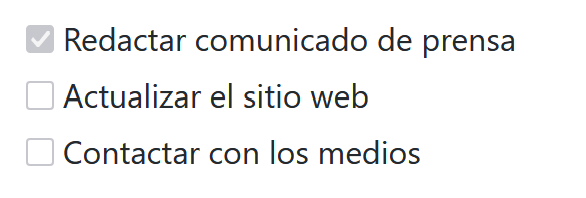
\includegraphics[scale=0.7]{images/tasklist}
	\vfill
\end{minipage}


\subsection{Añadir elementos a las listas}

Para añadir otro elemento a una lista manteniendo la continuidad de esta, indenta el elemento cuatro espacios o un tabulador, como se muestra en los ejemplos siguientes.

\medskip

\noindent \textbf{Consejo:} Si las cosas no aparecen como esperabas, comprueba que hayas indentado los elementos de la lista cuatro espacios o un tabulador.



\subsubsection{Párrafos}

\noindent
\begin{minipage}{0.5\textwidth}
\begin{lstlisting}[style=mdstyle]
* Primer elemento de la lista.
* Segundo elemento de la lista.

    Añado otro párrafo debajo del
    segundo elemento.

* Y tercer elemento de la lista.
\end{lstlisting}
\end{minipage}
~
\begin{minipage}{0.475\textwidth}
	\vfill
	\quad~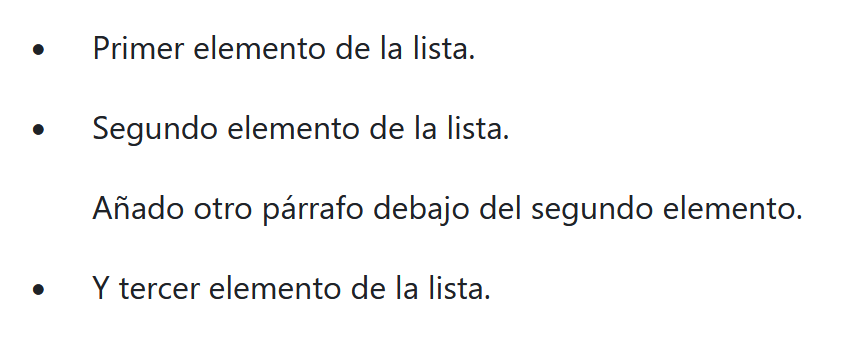
\includegraphics[scale=0.7]{images/list_paragraphs}
	\vfill
\end{minipage}

%El resultado será:
%* Este es el primer elemento de la lista.
%
%* Este es el segundo elemento de la lista.
%
%  Necesito añadir otro párrafo debajo del segundo elemento de la lista.
%
%* Y este es el tercer elemento de la lista.




\subsubsection{Citas en bloque}

\begin{lstlisting}[style=mdstyle]
* Este es el primer elemento de la lista.
* Este es el segundo elemento de la lista.

    > Una cita en bloque quedaría genial debajo del segundo elemento.

* Y este es el tercer elemento de la lista.
\end{lstlisting}

\medskip

\noindent El resultado será:

\bigskip

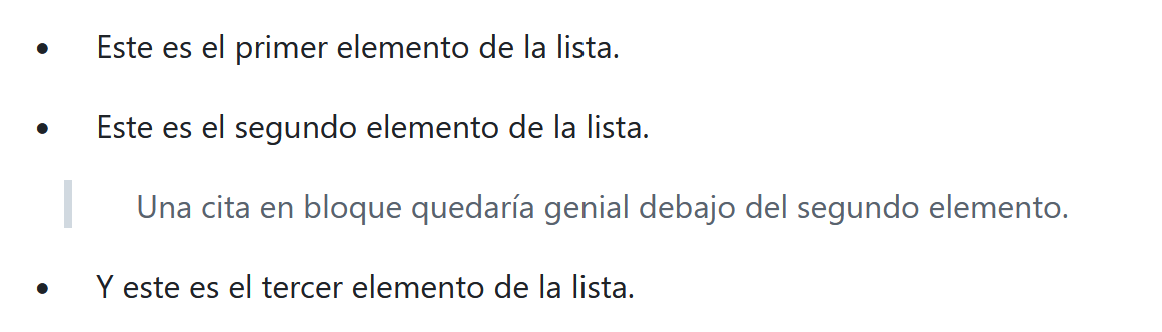
\includegraphics[scale=0.7]{images/list_blockquote}


%* Este es el primer elemento de la lista.
%* Este es el segundo elemento de la lista.
%
%  > Una cita en bloque quedaría genial debajo del segundo elemento de la lista.
%* Y este es el tercer elemento de la lista.







\subsubsection{Listas anidadas de diferentes tipos}

Puedes anidar una lista no ordenada dentro de una lista ordenada, o viceversa.

\bigskip

\noindent
\begin{minipage}{0.5\textwidth}
\begin{lstlisting}[style=mdstyle]
1. Primer elemento
2. Segundo elemento
3. Tercer elemento
    - Elemento indentado
    - Elemento indentado
4. Cuarto elemento
\end{lstlisting}
\end{minipage}
~
\begin{minipage}{0.475\textwidth}
	\vfill
	\quad~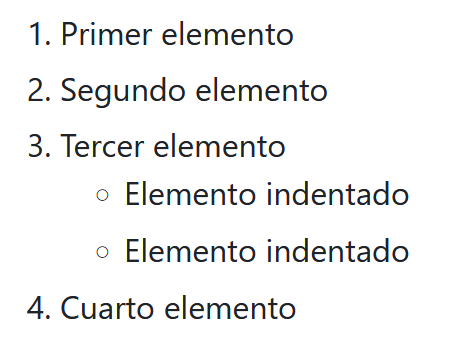
\includegraphics[scale=0.7]{images/list_of_lists}
	\vfill
\end{minipage}






\section{Código}

Para indicar que una palabra o frase es código, enciérrala entre comillas invertidas (\texttt{\textasciigrave...\textasciigrave}).

\bigskip

\noindent
\begin{minipage}{0.5\textwidth}
\begin{lstlisting}[style=mdstyle]
En el símbolo del sistema, escribe 
`nano`
\end{lstlisting}
\end{minipage}
~
\begin{minipage}{0.475\textwidth}
	\vfill
	\quad~
\includegraphics[scale=0.7]{images/code_1}
	\vfill
\end{minipage}


\subsection{Escapar comillas invertidas}

Si la palabra o frase que quieres indicar como código contiene una o más comillas invertidas, puedes escaparlas encerrando la palabra o frase entre dos comillas invertidas (\texttt{\textasciigrave\textasciigrave...\textasciigrave\textasciigrave}).

\bigskip

\noindent
\begin{minipage}{0.5\textwidth}
\begin{lstlisting}[style=mdstyle]
``Usa `code` en tu archivo Markdown.``
\end{lstlisting}
\end{minipage}
~
\begin{minipage}{0.475\textwidth}
	\vfill
	\quad~
\includegraphics[scale=0.7]{images/code_2}
	\vfill
\end{minipage}



\subsection{Bloques de código}

Para crear bloques de código, indenta cada línea del bloque al menos cuatro espacios o un tabulador.

\bigskip

\noindent
\begin{minipage}{0.5\textwidth}
\begin{lstlisting}[style=mdstyle]
    <html>
      <head>
      </head>
    </html>
\end{lstlisting}
\end{minipage}
~
\begin{minipage}{0.475\textwidth}
	\vfill
	\quad~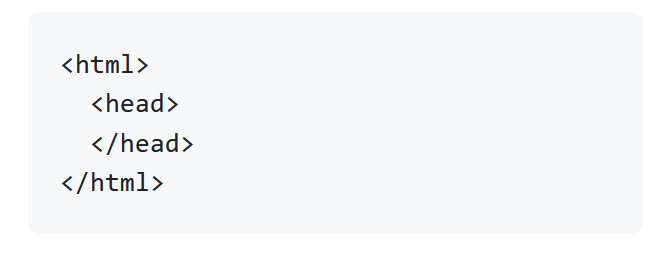
\includegraphics[scale=0.7]{images/code_3}
	\vfill
\end{minipage}

\noindent También podemos a crear bloques de código usando tres comillas invertidas (\texttt{\textasciigrave\textasciigrave\textasciigrave...\textasciigrave\textasciigrave\textasciigrave}).

\bigskip

\noindent
\begin{minipage}{0.5\textwidth}
\begin{lstlisting}[style=mdstyle]
```
<html>
	<head>
    </head>
</html>
```
\end{lstlisting}
\end{minipage}
~
\begin{minipage}{0.475\textwidth}
	\vfill
	\quad~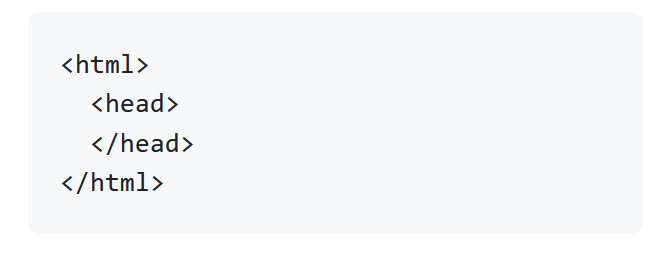
\includegraphics[scale=0.7]{images/code_3}
	\vfill
\end{minipage}

\bigskip

Algunos visualizadores de \Markdown\ permiten especificar el tipo de código y colorearlo acorde a las palabras clave reservadas. Por ejemplo, en \url{https://markdownviewer.pages.dev/} podemos especificar que nuestro código es de \R:

\bigskip

\noindent
\begin{minipage}{0.5\textwidth}
\begin{lstlisting}[style=mdstyle]
```-@R@-
f <- function-@()@- {
    print-@("Hola, mundo!")@-
}
```
\end{lstlisting}
\end{minipage}
~
\begin{minipage}{0.475\textwidth}
	\vfill
	\quad~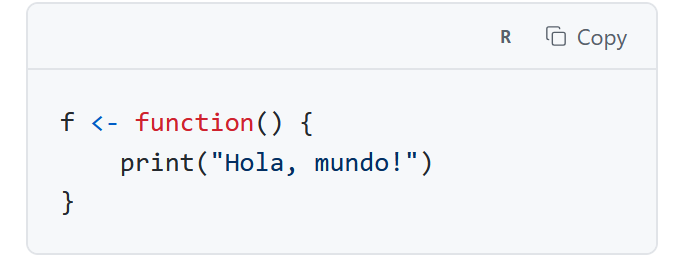
\includegraphics[scale=0.7]{images/code_4}
	\vfill
\end{minipage}




\subsection{Bloques de código}

Los bloques de código normalmente llevan una indentación de cuatro espacios o un tabulador. Cuando están dentro de una lista, indéntalos ocho espacios o dos tabuladores.

\begin{lstlisting}[style=mdstyle]
1. Abre el archivo.
2. Busca el siguiente bloque de código en la línea 21:

        <html>
          <head>
            <title>Test</title>
          </head>

3. Actualiza el título para que coincida con el nombre de tu sitio web.
\end{lstlisting}


\noindent El resultado será:

\medskip

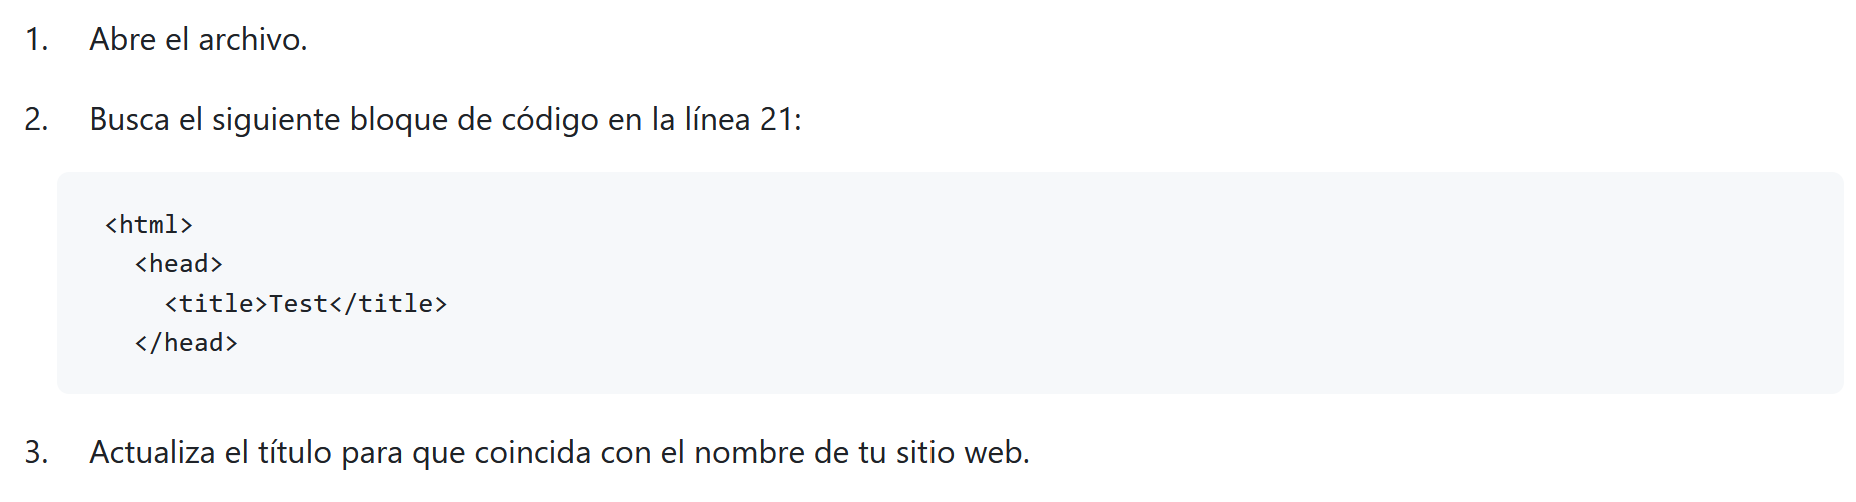
\includegraphics[scale=0.6]{images/code_5.png}

%1. Abre el archivo.
%
%2. Busca el siguiente bloque de código en la línea 21:
%
%   ```
%   <html>
%     <head>
%       <title>Test</title>
%     </head>
%   ```
%
%3. Actualiza el título para que coincida con el nombre de tu sitio web.




\section{Líneas horizontales}

Para crear una línea horizontal, utiliza tres o más asteriscos (\verb|***|), guiones (\verb|---|) o guiones bajos (\verb|___|) en una línea independiente.

\bigskip

\noindent
\begin{minipage}{0.5\textwidth}
\begin{lstlisting}[style=mdstyle]
Un texto

***

Otro texto

---

Otro

_________________
\end{lstlisting}
\end{minipage}
~
\begin{minipage}{0.475\textwidth}
	\vfill
	\quad~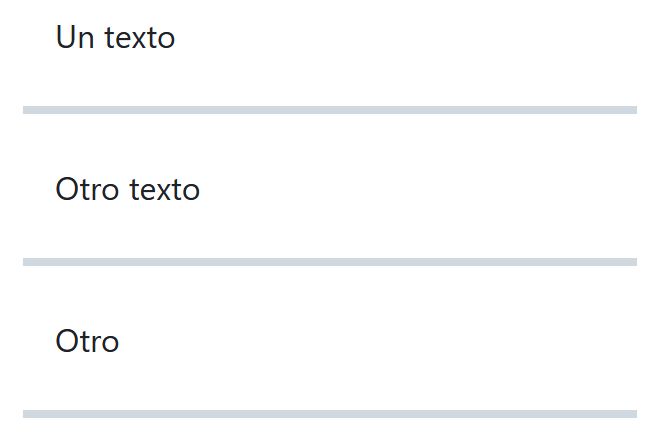
\includegraphics[scale=0.7]{images/rules}
	\vfill
\end{minipage}

\medskip

\noindent El resultado de las tres es idéntico.



\subsection{Buenas prácticas para las líneas horizontales}

Por compatibilidad, deja líneas en blanco antes y después de las líneas horizontales.


\begin{center}
\begin{tabular}{|l|l|} \hline
	\checkicon\ Haz esto & \crossicon\ No hagas esto \\ \hline
	
	\begin{tabular}{l}
		\\
		\verb|Pon una línea en blanco antes...| \\
		\\
		\verb|---| \\
		\\
		\verb|...y después de la línea horizontal.| \\
		\\
	\end{tabular}
	&
	\begin{tabular}{l}
		\\
		\verb|Sin líneas en blanco, esto sería| \\
		\verb|un encabezado.| \\
		\verb|---| \\
		\verb|¡No hagas esto!| \\
		\\
		\\
	\end{tabular}
	 \\ \hline
\end{tabular}
\end{center}





\section{Enlaces}

Para crear un enlace, encierra el texto del enlace entre corchetes (p. ej., \texttt{\textasciigrave[Duck Duck Go]\textasciigrave|}) y, justo después, añade la URL entre paréntesis (por ejemplo, \texttt{(https://duckduckgo.com)}).

\bigskip

\noindent
\begin{lstlisting}[style=mdstyle]
Mi buscador favorito es [Duck Duck Go](https://duckduckgo.com).
\end{lstlisting}

\noindent El resultado será:

\bigskip


\includegraphics[scale=0.7]{images/link}




\subsection{Añadir títulos}

Opcionalmente puedes añadir un título a un enlace. Este aparecerá como una información emergente cuando el usuario pase el cursor sobre el enlace. Para añadir un título, escríbelo entre comillas después de la URL.

\bigskip

\noindent
\begin{lstlisting}[style=mdstyle]
Mi buscador favorito es [Duck Duck Go](https://duckduckgo.com "El mejor
buscador para la privacidad").
\end{lstlisting}

\noindent El resultado será:

\bigskip


\includegraphics[scale=0.7]{images/link_title}




\subsection{URL y direcciones de correo electrónico}

Para convertir rápidamente una URL o una dirección de correo electrónico en un enlace, enciérrala entre corchetes angulares.

\bigskip

\noindent
\begin{minipage}{0.5\textwidth}
\begin{lstlisting}[style=mdstyle]
<https://www.markdownguide.org>

<fake@example.com>
\end{lstlisting}
\end{minipage}
~
\begin{minipage}{0.475\textwidth}
	\vfill
	\quad~
\includegraphics[scale=0.7]{images/mail}
	\vfill
\end{minipage}

\medskip

\noindent Mientras que el primero es un enlace a la página web, el segundo nos permite mandar un correo electrónico a esa dirección.



\subsection{Dar formato a los enlaces}

Para enfatizar los enlaces, añade asteriscos antes y después de los corchetes y paréntesis. Para indicar que un enlace es código, añade comillas invertidas dentro de los corchetes.

\bigskip

\begin{lstlisting}[style=mdstyle]
Me encanta apoyar a la **[EFF]-@(https://eff.org)@-**.

Este es el *-@[Markdown Guide](https://www.markdownguide.org)@-*.

Consulta la sección sobre [`code`]-@(\#code)@-.
\end{lstlisting}

\noindent El resultado será:

\bigskip

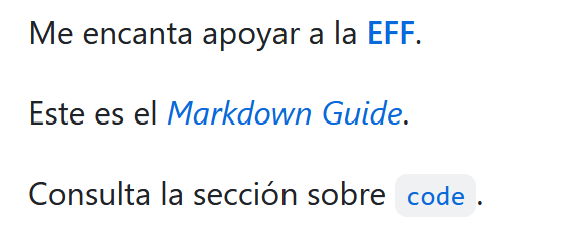
\includegraphics[scale=0.7]{images/emphasized_link}



%### Enlaces mediante referencias
%
%Los enlaces mediante referencias son un tipo especial de enlace que facilita la visualización y lectura de las URL en Markdown. Los enlaces mediante referencias se construyen en dos partes: la parte que mantienes integrada en el texto y la parte que almacenas en otro lugar del archivo para mantener el texto fácil de leer.
%
%\subsection{Dar formato a la primera parte del enlace}
%
%La primera parte de un enlace mediante referencia se escribe utilizando dos conjuntos de corchetes. El primer conjunto de corchetes contiene el texto que aparecerá como enlace. El segundo conjunto muestra una etiqueta que sirve para apuntar al enlace que has almacenado en otra parte del documento.
%
%Aunque no es obligatorio, puedes incluir un espacio entre el primer y el segundo conjunto de corchetes. La etiqueta del segundo conjunto no distingue entre mayúsculas y minúsculas y puede contener letras, números, espacios o signos de puntuación.
%
%Esto significa que los siguientes formatos son aproximadamente equivalentes para la primera parte del enlace:
%
%* `[hobbit-hole][1]`
%* `[hobbit-hole] [1]`
%
%\subsection{Dar formato a la segunda parte del enlace}
%
%La segunda parte de un enlace mediante referencia utiliza los siguientes atributos:
%
%1. La etiqueta, entre corchetes, seguida inmediatamente de dos puntos y al menos un espacio (por ejemplo, `[label]: `).
%2. La URL del enlace, que opcionalmente puedes encerrar entre corchetes angulares.
%3. El título opcional del enlace, que puedes encerrar entre comillas dobles, comillas simples o paréntesis.
%
%Esto significa que todos los ejemplos siguientes son aproximadamente equivalentes para la segunda parte del enlace:
%
%* `[1]: https://en.wikipedia.org/wiki/Hobbit#Lifestyle`
%* `[1]: https://en.wikipedia.org/wiki/Hobbit#Lifestyle "Estilos de vida de los hobbits"`
%* `[1]: https://en.wikipedia.org/wiki/Hobbit#Lifestyle 'Estilos de vida de los hobbits'`
%* `[1]: https://en.wikipedia.org/wiki/Hobbit#Lifestyle (Estilos de vida de los hobbits)`
%* `[1]: <https://en.wikipedia.org/wiki/Hobbit#Lifestyle> "Estilos de vida de los hobbits"`
%* `[1]: <https://en.wikipedia.org/wiki/Hobbit#Lifestyle> 'Estilos de vida de los hobbits'`
%* `[1]: <https://en.wikipedia.org/wiki/Hobbit#Lifestyle> (Estilos de vida de los hobbits)`
%
%Puedes colocar esta segunda parte en cualquier lugar del documento Markdown. Algunas personas la colocan inmediatamente después del párrafo en el que aparece, mientras que otras la sitúan al final del documento, como si fueran notas finales o notas al pie.
%
%#### Un ejemplo que combina las dos partes
%
%Supongamos que añades una URL como [enlace URL estándar](https://www.markdownguide.org/basic-syntax/#links) a un párrafo y queda así en Markdown:
%
%```text
%En un agujero en el suelo vivía un hobbit. No era un agujero desagradable, sucio y mojado,
%lleno de restos de gusanos y con un olor a humedad, ni tampoco un agujero seco, desnudo y
%arenoso sin nada donde sentarse o comer: era un [agujero-hobbit](https://en.wikipedia.org/wiki/Hobbit#Lifestyle "Estilos de vida de los hobbits"), y eso significa comodidad.
%```
%
%Aunque puede dirigir a información adicional interesante, la URL mostrada realmente no aporta mucho al texto original, aparte de dificultar su lectura. Para solucionarlo, puedes escribir la URL de esta manera:
%
%```text
%En un agujero en el suelo vivía un hobbit. No era un agujero desagradable, sucio y mojado,
%lleno de restos de gusanos y con un olor a humedad, ni tampoco un agujero seco, desnudo y
%arenoso sin nada donde sentarse o comer: era un [agujero-hobbit][1], y eso significa comodidad.
%
%[1]: <https://en.wikipedia.org/wiki/Hobbit#Lifestyle> "Estilos de vida de los hobbits"
%```
%
%En ambos casos, el resultado visual sería idéntico:
%
%> En un agujero en el suelo vivía un hobbit. No era un agujero desagradable, sucio y mojado, lleno de restos de gusanos y con un olor a humedad, ni tampoco un agujero seco, desnudo y arenoso sin nada donde sentarse o comer: era un [agujero-hobbit](https://en.wikipedia.org/wiki/Hobbit#Lifestyle "Estilos de vida de los hobbits"), y eso significa comodidad.
%
%Y el HTML del enlace sería:
%
%```html
%<a href="https://en.wikipedia.org/wiki/Hobbit#Lifestyle" title="Estilos de vida de los hobbits">agujero-hobbit</a>
%```









\subsection{Buenas prácticas para los enlaces}

Las aplicaciones de Markdown no se ponen de acuerdo sobre cómo gestionar los espacios dentro de una URL. Por compatibilidad, intenta codificar los espacios de la URL utilizando \verb|%20|. Como alternativa, si tu aplicación de Markdown admite HTML, puedes utilizar la etiqueta HTML \verb|a|.


\begin{center}
\begin{tabular}{|l|l|} \hline
	\checkicon\ Haz esto & \crossicon\ No hagas esto \\ \hline
	
	\begin{tabular}{l}
		\\
		\verb|[enlace](https://www.example.com/| \\
		\verb|my%20great%20page)| \\
		\\
		\verb|<a href="https://www.example.com/| \\
		\verb|my great page">enlace</a>| \\
		\\
	\end{tabular}
	&
	\begin{tabular}{l}
		\\
		\\
		\verb|[enlace](https://www.example.com/| \\
		\verb|my great page)| \\
		\verb|    | \\
		\verb|    | \\
		\\
	\end{tabular}
	 \\ \hline
\end{tabular}
\end{center}

Los paréntesis dentro de una URL también pueden causar problemas. Por compatibilidad, intenta codificar el paréntesis de apertura (\verb|(|) como \verb|%28| y el de cierre (\verb|)|) como \verb|%29|. Como alternativa, si tu aplicación de Markdown admite HTML, puedes utilizar la etiqueta HTML \verb|a|.

\begin{center}
\begin{tabular}{|l|l|} \hline
	\checkicon\ Haz esto & \crossicon\ No hagas esto \\ \hline
	
	\begin{tabular}{l}
		\\
		\footnotesize\verb|[una novela](https://en.wikipedia.org/| \\
		\footnotesize\verb|wiki/The_Milagro_Beanfield_War_%28novel%29)| \\
		\\
		\footnotesize\verb|<a href="https://en.wikipedia.org/| \\
		\footnotesize\verb|wiki/The_Milagro_Beanfield_War_(novel)">| \\
		\footnotesize\verb|una novela</a>| \\
		\\
	\end{tabular}
	&
	\begin{tabular}{l}
		\\
		\\
		\footnotesize\verb|[una novela](https://en.wikipedia.org/| \\
		\footnotesize\verb|wiki/The_Milagro_Beanfield_War_(novel))| \\
		\verb|    | \\
		\verb|    | \\
		\\
		\\
	\end{tabular}
	 \\ \hline
\end{tabular}
\end{center}





\section{Imágenes}

Para añadir una imagen, añade un signo de exclamación (\verb|!|), seguido del texto alternativo entre corchetes y de la ruta o URL del recurso de imagen entre paréntesis. Opcionalmente puedes añadir un título entre comillas después de la ruta o URL.

\begin{lstlisting}[style=mdstyle]
![Las montañas de San Juan son preciosas](/assets/images/san-juan-mountains.jpg "Montañas de San Juan")
\end{lstlisting}


\noindent El resultado será:

\begin{center}
	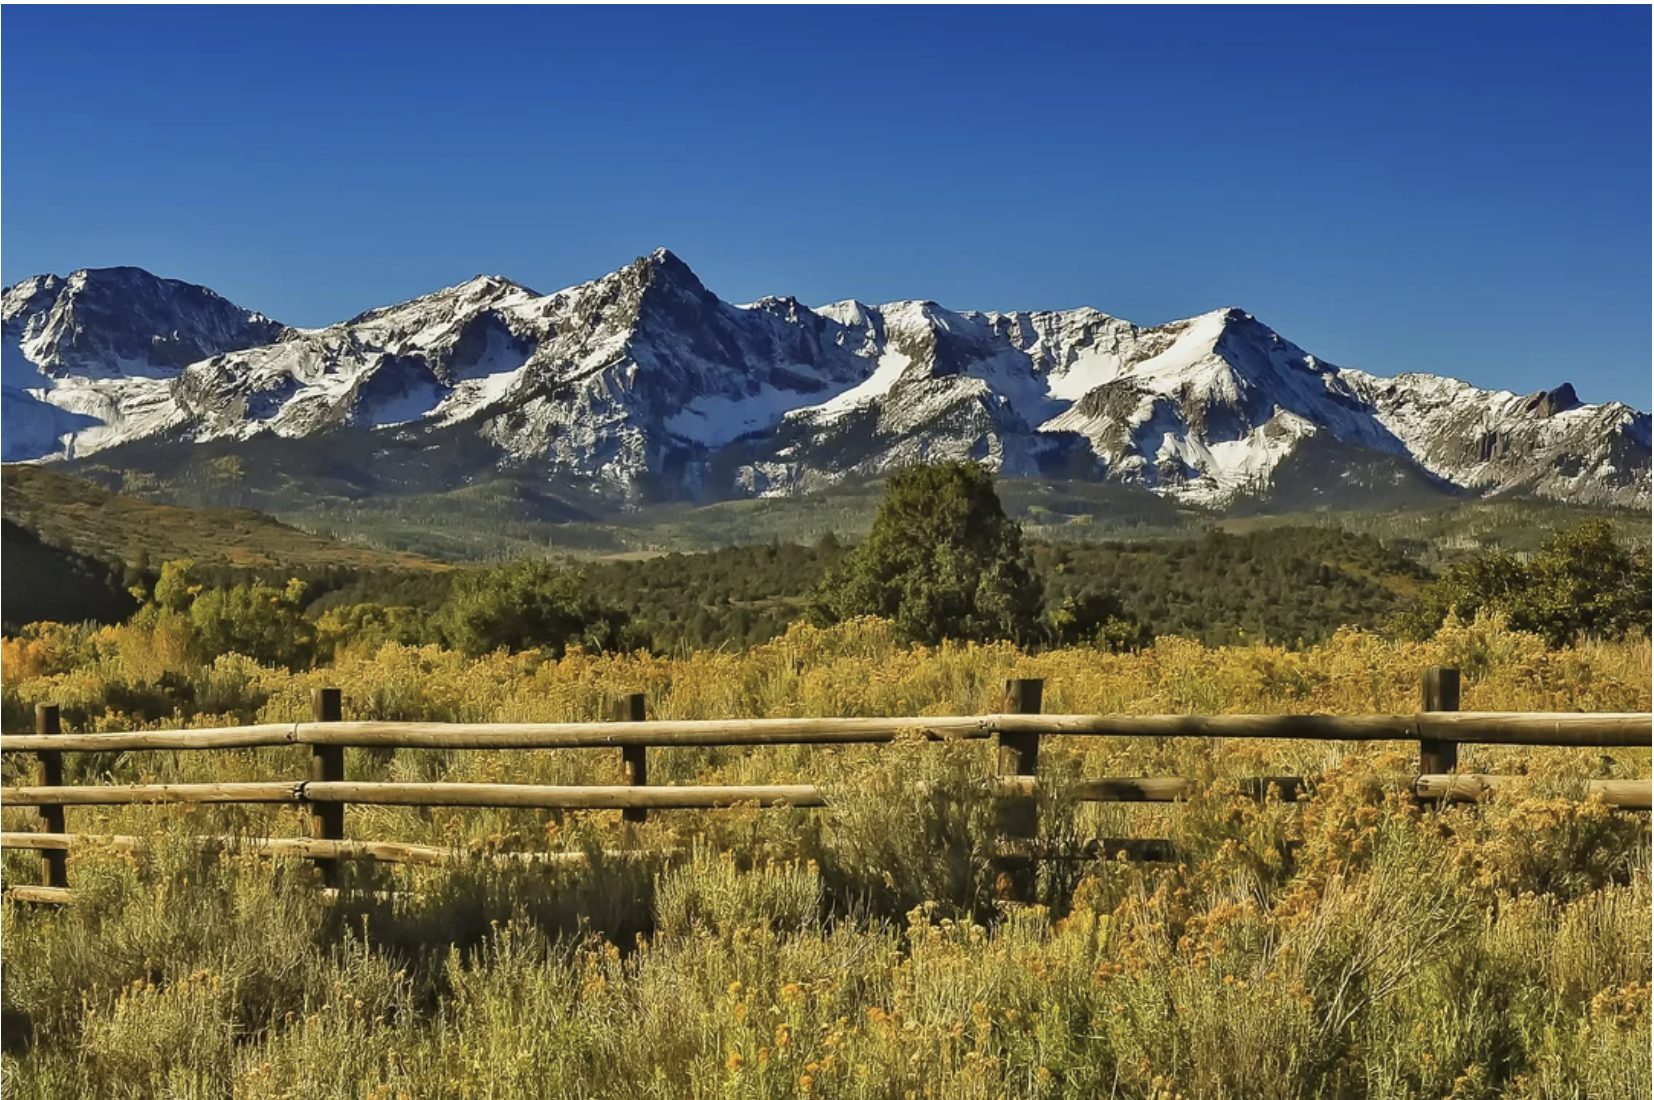
\includegraphics[scale=0.5]{images/image_1}
\end{center}



\subsection{Enlazar imágenes}

Para añadir un enlace a una imagen, encierra el código Markdown de la imagen entre corchetes y después añade el enlace entre paréntesis.


\begin{lstlisting}[style=mdstyle]
[![Una roca antigua en el desierto](/assets/images/shiprock.jpg "Shiprock, Nuevo México, por Beau Rogers")](https://www.flickr.com/photos/beaurogers/31833779864/in/photolist-Qv3rFw-34mt9F-a9Cmfy-5Ha3Zi-9msKdv-o3hgjr-hWpUte-4WMsJ1-KUQ8N-deshUb-vssBD-6CQci6-8AFCiD-zsJWT-nNfsgB-dPDwZJ-bn9JGn-5HtSXY-6CUhAL-a4UTXB-ugPum-KUPSo-fBLNm-6CUmpy-4WMsc9-8a7D3T-83KJev-6CQ2bK-nNusHJ-a78rQH-nw3NvT-7aq2qf-8wwBso-3nNceh-ugSKP-4mh4kh-bbeeqH-a7biME-q3PtTf-brFpgb-cg38zw-bXMZc-nJPELD-f58Lmo-bXMYG-bz8AAi-bxNtNT-bXMYi-bXMY6-bXMYv)
\end{lstlisting}


\noindent El resultado es una imagen que al clickar sobre ella nos llevará a la página enlazada:


\begin{center}
	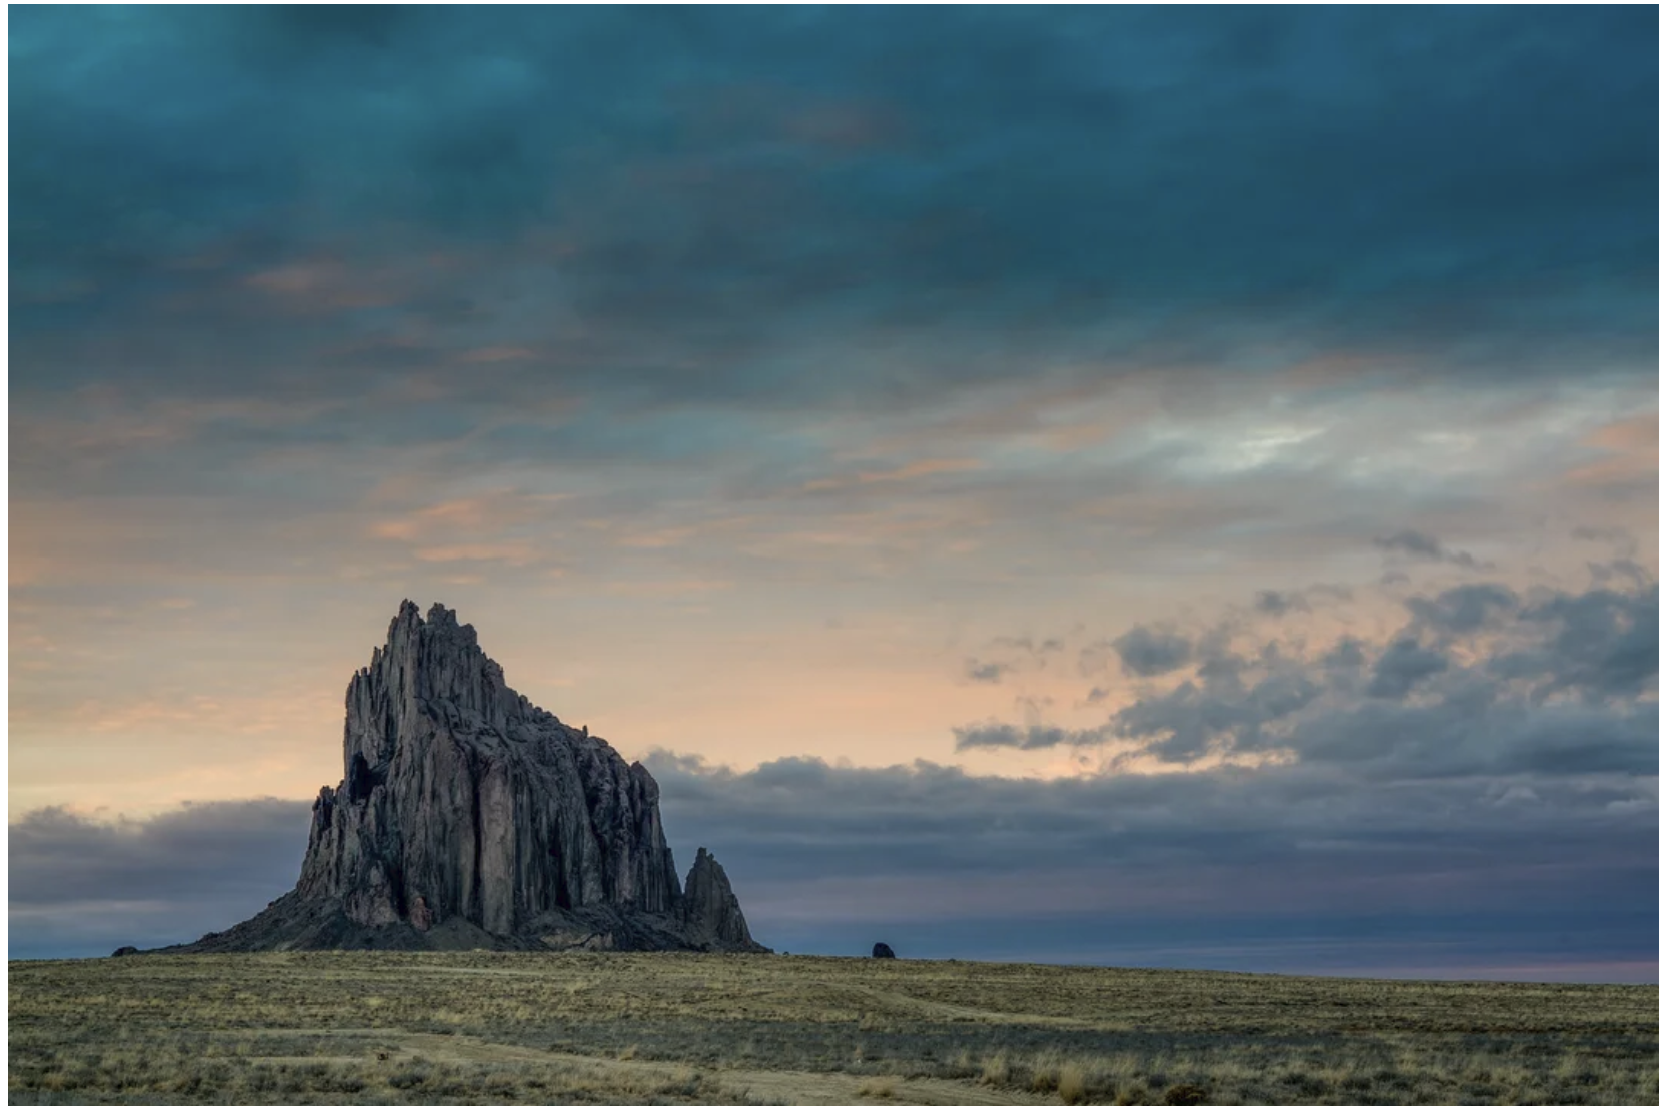
\includegraphics[scale=0.45]{images/image_2}
\end{center}




\subsection{Lista con imágenes}

Podemos incluir imágenes en listas:


\noindent
\begin{minipage}{0.5\textwidth}
\begin{lstlisting}[style=mdstyle]
1. Open the file containing the
Linux mascot.
2. Marvel at its beauty.

    ![Tux, the Linux mascot]
    -@(/assets/images/tux.png)@-

3. Close the file.
\end{lstlisting}
\end{minipage}
~
\begin{minipage}{0.475\textwidth}
	\vfill
	\quad~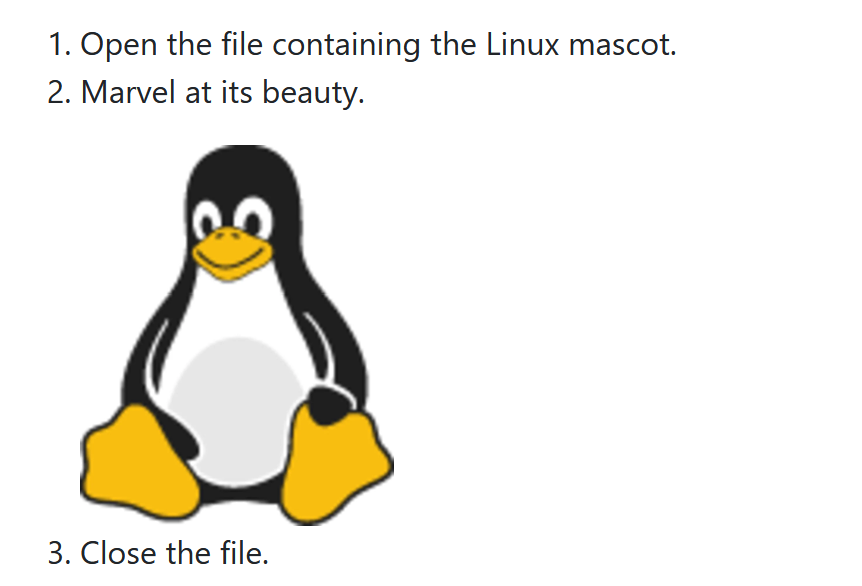
\includegraphics[scale=0.6]{images/list_image}
	\vfill
\end{minipage}




\section{Caracteres de escape}

Para mostrar literalmente un carácter que, de otro modo, se utilizaría para dar formato al texto en un documento Markdown, añade una barra invertida (\verb|\|) delante del carácter.

\bigskip

\begin{lstlisting}[style=mdstyle]
\* Sin la barra invertida, esto sería una viñeta de una lista no ordenada.
\end{lstlisting}

\medskip

\noindent El resultado será:

\begin{center}

\includegraphics[scale=0.75]{images/scaping}
\end{center}


\subsection{Caracteres que puedes escapar}

Puedes utilizar una barra invertida para escapar los siguientes caracteres.

\begin{center}
\begin{tabular}{|c|l|} \hline
	Carácter & Nombre \\ \hline
	\verb|\| & barra invertida \\
	\texttt{\textasciigrave} & comilla invertida \\
	\verb|*| & asterisco \\ 
	\verb|_| & guion bajo \\
	\verb|{ }| & llaves \\
	\verb|[ ]| & corchetes \\
	\verb|< >| & corchetes angulares \\ \hline
\end{tabular}
~
\quad
~
\begin{tabular}{|c|l|} \hline
	Carácter & Nombre \\ \hline
	\verb|( )| & paréntesis \\
	\verb|#| & almohadilla \\
	\verb|+| & signo más \\
	\verb|-| & signo menos (guion) \\ 
	\verb|.| & punto \\
	\verb|!| & signo de exclamación \\
	\texttt{|} & barra vertical \\ \hline
\end{tabular}
\end{center}



\section{HTML}

Muchas aplicaciones de \Markdown\ permiten utilizar etiquetas HTML en texto con formato \Markdown. Esto resulta útil si prefieres determinadas etiquetas HTML a la sintaxis de \Markdown. Por ejemplo, algunas personas consideran más sencillo utilizar etiquetas HTML para las imágenes. Utilizar HTML también resulta útil cuando necesitas cambiar los atributos de un elemento, como especificar el color del texto o modificar el ancho de una imagen. Para utilizar HTML, coloca las etiquetas en el texto de tu archivo con formato Markdown.

\bigskip

\noindent
\begin{minipage}{0.5\textwidth}
\begin{lstlisting}[style=mdstyle]
Esta **palabra** está en negrita. 

Esta <em>palabra</em> está en cursiva.
\end{lstlisting}
\end{minipage}
~
\begin{minipage}{0.475\textwidth}
	\vfill
	\quad~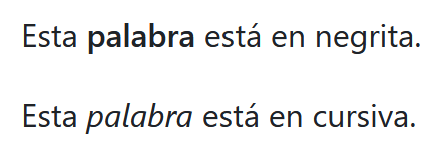
\includegraphics[scale=0.7]{images/html}
	\vfill
\end{minipage}


\subsection{Buenas prácticas para HTML}

Por motivos de seguridad, no todas las aplicaciones de \Markdown\ admiten HTML en documentos \Markdown. En caso de duda, consulta la documentación de tu aplicación de \Markdown. Algunas aplicaciones solo admiten un subconjunto de las etiquetas HTML.

\medskip

Utiliza líneas en blanco para separar los elementos HTML a nivel de bloque, como \verb|<div>|, \verb|<table>|, \verb|<pre>| y \verb|<p>|, del contenido que los rodea. Intenta no indentar las etiquetas con tabuladores o espacios, ya que esto puede interferir con el formato. No puedes utilizar sintaxis \Markdown\ dentro de etiquetas HTML a nivel de bloque. Por ejemplo,

\medskip

\begin{lstlisting}[style=mdstyle]
<p>cursiva y **negrita**</p>
\end{lstlisting}

\medskip

\noindent no funcionará.




\newpage
\section{Ejercicios}


\begin{exercise} Escribe un fichero \texttt{README.md} en la raíz de tu repositorio de prácticas y un directorio llamado \texttt{assets}, y dentro de este un directorio que se llame \texttt{images}. Observa que tendremos dos ficheros \texttt{README.md}, el del directorio \texttt{Git} y el nuevo.

\begin{center}
\begin{minipage}{0.75\linewidth}
\dirtree{%
    .1 \faIcon[regular]{folder-open}\ practicas/.
	    .2 \faIcon[regular]{folder-open}\ .git/.
        .2 \faIcon[regular]{folder-open}\ .gitignore.
        .2 \faIcon[regular]{folder-open}\ assets/.
            .3 \faIcon[regular]{folder-open}\ images/.
        .2 \faIcon[regular]{folder-open}\ Git/.
            .3 \faIcon[regular]{file-alt}\ README.md.
        .2 \faIcon[regular]{folder-open}\ R/.
            .3 \faIcon[regular]{folder-open}\ practica\_1/.
                .4 \faIcon[regular]{file-alt}\ ej1.R.
                .4 ....
            .3 \faIcon[regular]{folder-open}\ practica\_3/.
                .4 \faIcon[regular]{file-alt}\ ej1.R.
                .4 ....
            .3 ....
        .2 \faIcon[regular]{file-alt}\ README.md.
}
\end{minipage}
\end{center}

\bigskip

\noindent El contenido de dicho fichero se muestra en la siguiente página. Algunas aclaraciones:
\begin{enumerate}
	\item Intenta imitar todo lo relativo al formato: encabezados, negrita, cursiva, etc.
	\item Deberás incluir una cita sobre las matemáticas que te guste y que sea distinta a la que aparece en la imagen.
	\item Completa las listas. No dejes puntos suspensivos (\texttt{...}) en ellas. 
	\item Añade una imagen que te guste (podría ser la imagen del enunciado si te gusta, pero tendrás que buscarla en internet).
	\item Aquellas expresiones en azul son enlaces. Pon los enlaces correctos. Además, en el apartado \textbf{Herramientas necesarias}, añade más detalles sobre la descarga e instalación.
	\item En el apartado \textbf{Autor/Autora} deberás escribir tu nombre.
	\item La imagen del final deberá ser una imagen con enlace a la página oficial del CEU Cardenal Herrera.
\end{enumerate}

\noindent Sube a tu repositorio de \GitHub\ el \texttt{README.md} y comprueba que se ve correctamente.

\begin{center}

\includegraphics[scale=1]{images/readme_1}
\end{center}
\end{exercise}


\newpage
\begin{exercise} En los directorios donde tengas los ficheros de las prácticas 1 y 3, añade un fichero \texttt{README.md}, que tenga el aspecto que se muestra abajo. Algunas aclaraciones:
\begin{enumerate}
	\item Añade el título de la práctica (mira el \texttt{.pdf} correspondiente) y añade una descripción que permita saber el objetivo de la práctica.
	\item Deberás añadir una breve descripción del objetivo de cada ejercicio. No es necesario que elabores mucho esta descripción, ya que tus ficheros estarán lo suficientemente comentados como para saber que ocurre en cada uno.
	\item Completa las listas. No dejes puntos suspensivos (\texttt{...}) en ellas. Podría pasar que algún fichero tenga más de un ejercicio resuelto. No pasa nada. Si quisieras separarlos en varios ficheros, es un buen momento. 
\end{enumerate}

\vfill
\begin{center}
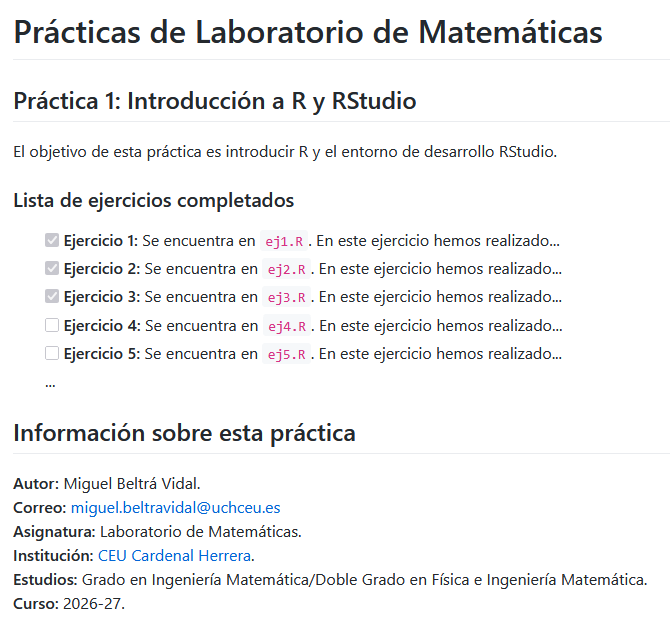
\includegraphics[scale=1]{images/readme_2}
\end{center}
\vfill
\end{exercise}




\newpage
\begin{exercise} En el directorio donde tengas la práctica 2, añade un fichero \texttt{README.md}, que tenga el aspecto que se muestra abajo.

\vfill
\begin{center}
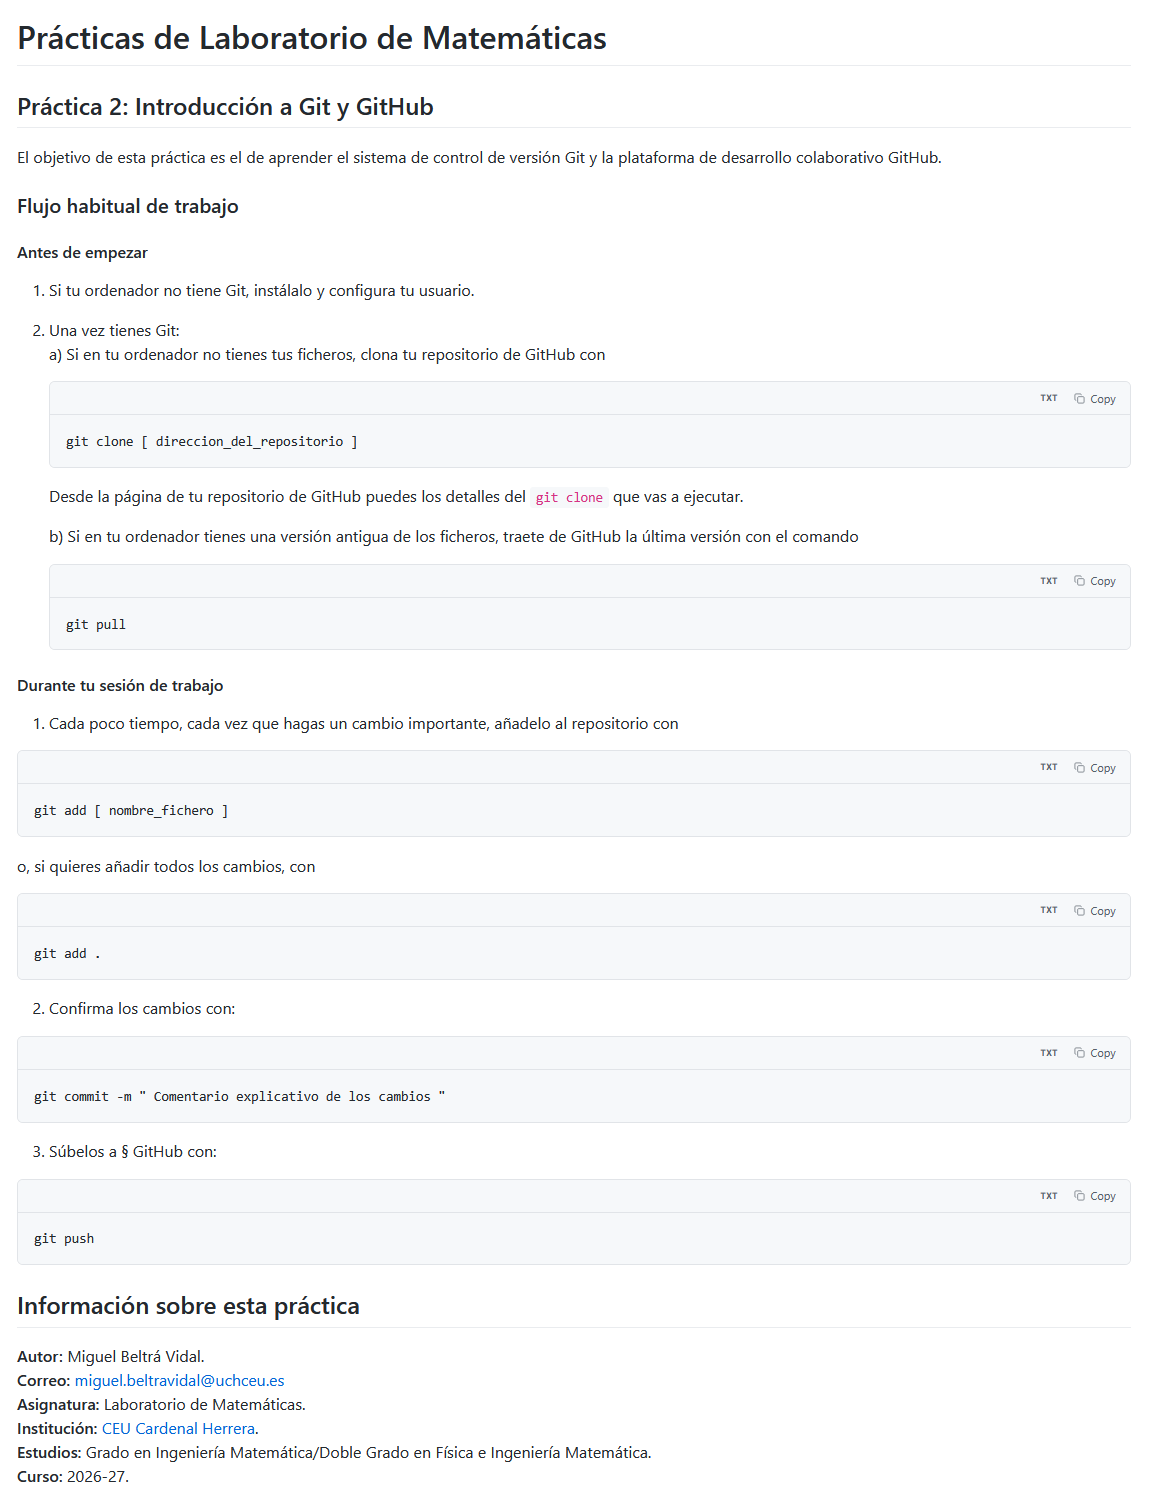
\includegraphics[scale=0.85]{images/readme_3}
\end{center}
\vfill
\end{exercise}


\section{Entrega y consejos}

Sube tus ficheros a \GitHub\ antes de la fecha concretada con el profesor. Trata de seguir las buenas prácticas. Utiliza previsualizadores para comprobar que todo está bien. Revisa en \GitHub\ que los ficheros \texttt{README.md} se renderizan correctamente. A partir de este momento, deberás llevar a cabo un mantenimiento de estos ficheros \texttt{README.md}, actualizándolos siempre que sea necesario.


\end{document}